\chapter{非断熱遷移}\label{NT}
本章では,量子力学における非断熱遷移に関連する内容を説明する.特に,非断熱遷移では,幾何学的な量が重要な役割を担う.


\section{序論}
断熱状態間の遷移を非断熱遷移(nonadiabatic transition)と呼ぶ。非断熱遷移では,ある種の幾何学的位相が遷移確率に寄与することを以下で示そう。


第2章と同様に,2準位系のHermiteなHamiltonianを
\begin{align}
  \Hat{H}(t)
  &:= x(t)\Hat{\sigma}_x + y(t) \Hat{\sigma}_y + z(t) \Hat{\sigma}_z\\
  &=
  \begin{pmatrix} 
  z(t) & x(t) - iy(t)\\
  x(t) + iy(t) & -z(t)\\
  \end{pmatrix}\\
  &= E_2(t)
  \begin{pmatrix} 
  \cos \theta(t) & \sin \theta(t) \exp(-i\phi(t))\\
  \sin \theta(t) \exp(+i\phi(t)) & -\cos \theta(t)\\
  \end{pmatrix}
\end{align}
とする.ただし,直交座標$\{x(t), y(t), z(t)\}$から極座標$\{E_2(t), \theta(t), \phi(t)\}$への変換式
\begin{align}
  x(t) &= E_2(t) \sin \theta(t) \cos \phi(t)\\
  y(t) &= E_2(t) \sin \theta(t) \sin \phi(t)\\
  z(t) &= E_2(t) \cos \theta(t)
\end{align}
を用いた.


断熱パラメータ$\delta$を定義して,$t = \delta \tau$とする.$\delta$が非常に小さいときは,断熱近似ができる.ここで,
\begin{align}
  |\psi(\tau)\rangle = \exp \left( -\frac{i}{\hbar} \int_0^{\tau} d\tau^{\prime} E_2(\delta \tau^{\prime}) \right) |\phi_2(\delta \tau) \rangle
\end{align}
を仮定する.ただし,$| \phi_2(t) \rangle$は,式(\ref{EE})を満たす断熱状態
\begin{equation}
  | \phi_2(t) \rangle
  = \exp(i\mu(t))
  \begin{pmatrix}
    \cos(\frac{\theta(t)}{2})\exp(-i\frac{\phi(t)}{2})\\[8pt]
    \sin(\frac{\theta(t)}{2})\exp(+i\frac{\phi(t)}{2})
  \end{pmatrix}
\end{equation}
である.任意定数$\mu(t)$を決定するために,平行移動条件(parallel transport requirement)
\begin{equation}
  \langle \phi_2 | \Dot{\phi}_2 \rangle = 0
\end{equation}
を仮定すると,
\begin{equation}
  \mu(t) = \frac{1}{2} \int_0^{t} dt^{\prime} \Dot{\phi} \cos\theta = \frac{1}{2} \int_0^{t} dt^{\prime} \frac{(x\Dot{y}-y\Dot{x})z}{(x^2+y^2)\sqrt{x^2+y^2+z^2}} 
\end{equation}
となる.$\mu(t)$を幾何学的位相(geometric phase)と呼ぶ.


$\mu(t)$が非断熱遷移の確率にどのような影響を与えるか調べよう.そのためのもっとも簡単な方法はDykhne-Davis-Pechukas(DDP)法を用いることである\footnote{Dykhne-Davis-Pechukas(DDP)法は,Dykhne公式と呼ぶこともある.}\cite{Dykhne}\cite{DavisPechukas1976}\cite{Hwang}.DDP法は,任意の実対称Hamiltonianで記述される系における非断熱遷移の確率を与える強力な公式である.しかし,今は複素Hamiltonianを考えているから,ただちにDDP法を用いることはできない.そのため,適当なユニタリ変換によってHamiltonianを実対称化する.

また,ユニタリ演算子
\begin{equation}
  \Hat{U}:=
  \begin{pmatrix} 
    \exp(-i\frac{1}{2} \phi(t))&0\\
    0&\exp(i\frac{1}{2} \phi(t))\\
  \end{pmatrix}
\end{equation}
を定義する.このとき,
\begin{align}
  \Hat{U}^{\dagger} \Hat{H} \Hat{U}
  &=
  \begin{pmatrix}
    e^{-i\frac{\phi}{2}} & 0\\
    0 & e^{i\frac{\phi}{2}}\\
  \end{pmatrix}
  \begin{pmatrix}
    z & x-iy\\
    x+iy & -z\\
  \end{pmatrix}
  \begin{pmatrix}
    e^{i\frac{\phi}{2}} & 0\\
    0 & e^{-i\frac{\phi}{2}}\\
  \end{pmatrix}\\
  &=
  \begin{pmatrix}
   z & e^{-i\phi} (x-iy)\\
    e^{i\phi} (x+iy) & -z\\
  \end{pmatrix}\\
  &=
  \begin{pmatrix}
   z & e^{-i\phi} (E_2\sin\theta e^{i\phi})\\
    e^{i\phi} (E_2\sin\theta e^{-i\phi}) & -z\\
  \end{pmatrix}\\
  &=
  \begin{pmatrix}
   z & \sqrt{x^2+y^2}\\
   \sqrt{x^2+y^2} & -z\\
  \end{pmatrix}
\end{align}
となる.ここで,$|\psi_{\mathrm{LZ}}(t) \rangle := \Hat{U}^{\dagger} |\psi(t) \rangle$とすると,Shr\"{o}dinger方程式(\ref{SE})は,
\begin{equation}
  \Hat{H} \Hat{U} |\psi_{\mathrm{LZ}}(t) \rangle = i \hbar \frac{\partial}{\partial t} (\Hat{U} |\psi_{\mathrm{LZ}}(t) \rangle)
\end{equation}
となる.左から$\Hat{U}^{\dagger}$をかけると,
\begin{equation}
  \Hat{U}^{\dagger} \Hat{H} \Hat{U} |\psi_{\mathrm{LZ}}(t) \rangle = i \hbar \left(\Hat{U}^{\dagger} \frac{\partial}{\partial t} \Hat{U} \right)|\psi_{\mathrm{LZ}}(t) \rangle + i \hbar \frac{\partial}{\partial t} |\psi_{\mathrm{LZ}}(t) \rangle \label{SE_LZ1}
\end{equation}
となる.また,ユニタリ変換後のHamiltonian $H_{\mathrm{LZ}}$および$|\psi_{\mathrm{LZ}}(t) \rangle := U^{\dagger} |\psi(t) \rangle$に対して,Shr\"{o}dinger方程式
\begin{equation}
  \Hat{H}_{\mathrm{LZ}}(t) |\psi_{\mathrm{LZ}}(t) \rangle = i\hbar \frac{\partial}{\partial t} |\psi_{\mathrm{LZ}}(t) \rangle  \label{SE_LZ}
\end{equation} 
が成り立つから,式(\ref{SE_LZ1})に,式(\ref{SE_LZ})を代入して整理すると,
\begin{equation}
  \Hat{H}_{\mathrm{LZ}}(t)  = \Hat{U}^{\dagger} \Hat{H} \Hat{U} - i\hbar \Hat{U}^{\dagger} \frac{\partial}{\partial t} \Hat{U} 
\end{equation}
が得られる.これを計算すると,ユニタリ変換後のHamiltonian $H_{\mathrm{LZ}}$は,
\begin{equation}
  \Hat{H}_{\mathrm{LZ}}(t) =
  \begin{pmatrix}
    \left(z - \hbar \frac{\partial_t \phi}{2} \frac{dt}{d\tau}\right) & \sqrt{x^2+y^2}\\
    \sqrt{x^2+y^2} & -\left(z - \hbar \frac{\partial_t \phi}{2} \frac{dt}{d\tau}\right)
  \end{pmatrix}
\end{equation}
となる.したがって,複素Hamiltonian $H$を,実対称Hamiltonian $H_{\mathrm{LZ}}$に変換することができた.


ここで,DDP法を用いると,非断熱遷移の確率
\begin{equation}
  P \approx \exp \left(\frac{4}{\delta \hbar} \mathrm{Im} \int_0^{t_c} E_{\mathrm{LZ}_2} dt \right) \label{P_nt}\\
\end{equation}
が得られる.ただし,$E_{\mathrm{LZ}_2}$は,変換後の系における高い方の断熱エネルギーであり,
\begin{equation}
  E_{\mathrm{LZ}_2} 
  = \sqrt{\left(z - \frac{1}{2} \hbar \delta \Dot{\phi}\right)^2 + x^2+y^2} \label{E_LZ}
\end{equation}
である.また,$t_c \in \mathbb{C}$は,$E_{\mathrm{LZ}_2} = 0$となる虚時間を表す.

式(\ref{P_nt})に$E_{\mathrm{LZ}_2}$を代入すると,$\delta \ll 1$のとき,
\begin{equation}
  P \approx \exp\left(-\frac{4}{\hbar \delta} \left|\,\mathrm{Im} \int_0^{t_c} dt E_2(t) \right|-2\,\mathrm{Im} \int_0^{t_c} dt \frac{\Dot{\phi} z}{E_2(t)} \right)
\end{equation}
となる.第1項は動力学的位相の寄与(dynamical exponent)$\Gamma_d$,第2項は幾何学的位相の寄与(geometric exponent)$\Gamma_g$である.$\Gamma_d$は,$\hbar$や$\delta$という量に依存するのに対して,$\Gamma_g$はパラメータ空間の座標変数とその時間微分のみに依存するという意味で幾何学的であるといえる.


$\Gamma_g$が幾何学的な量であること別の方法で確かめてみよう.そのために,図\ref{fig:solidangle_GP}のような経路で複素積分を行う.すると,
\begin{equation}
  \Gamma_g = -\frac{1}{2} \, \mathrm{Im} \oint dt \Dot{\phi} \cos \theta = -\frac{1}{2} \, \mathrm{Im} \oint d\phi \cos \theta \label{gamma_g_solid}
\end{equation}
となる.この式は,$\Gamma_g$が複素Hamiltonianのパラメータ空間における立体角として解釈できることを示唆している.すなわち,$\Gamma_g$は幾何学的な量である.

\begin{figure}[htbp]
  \centering
  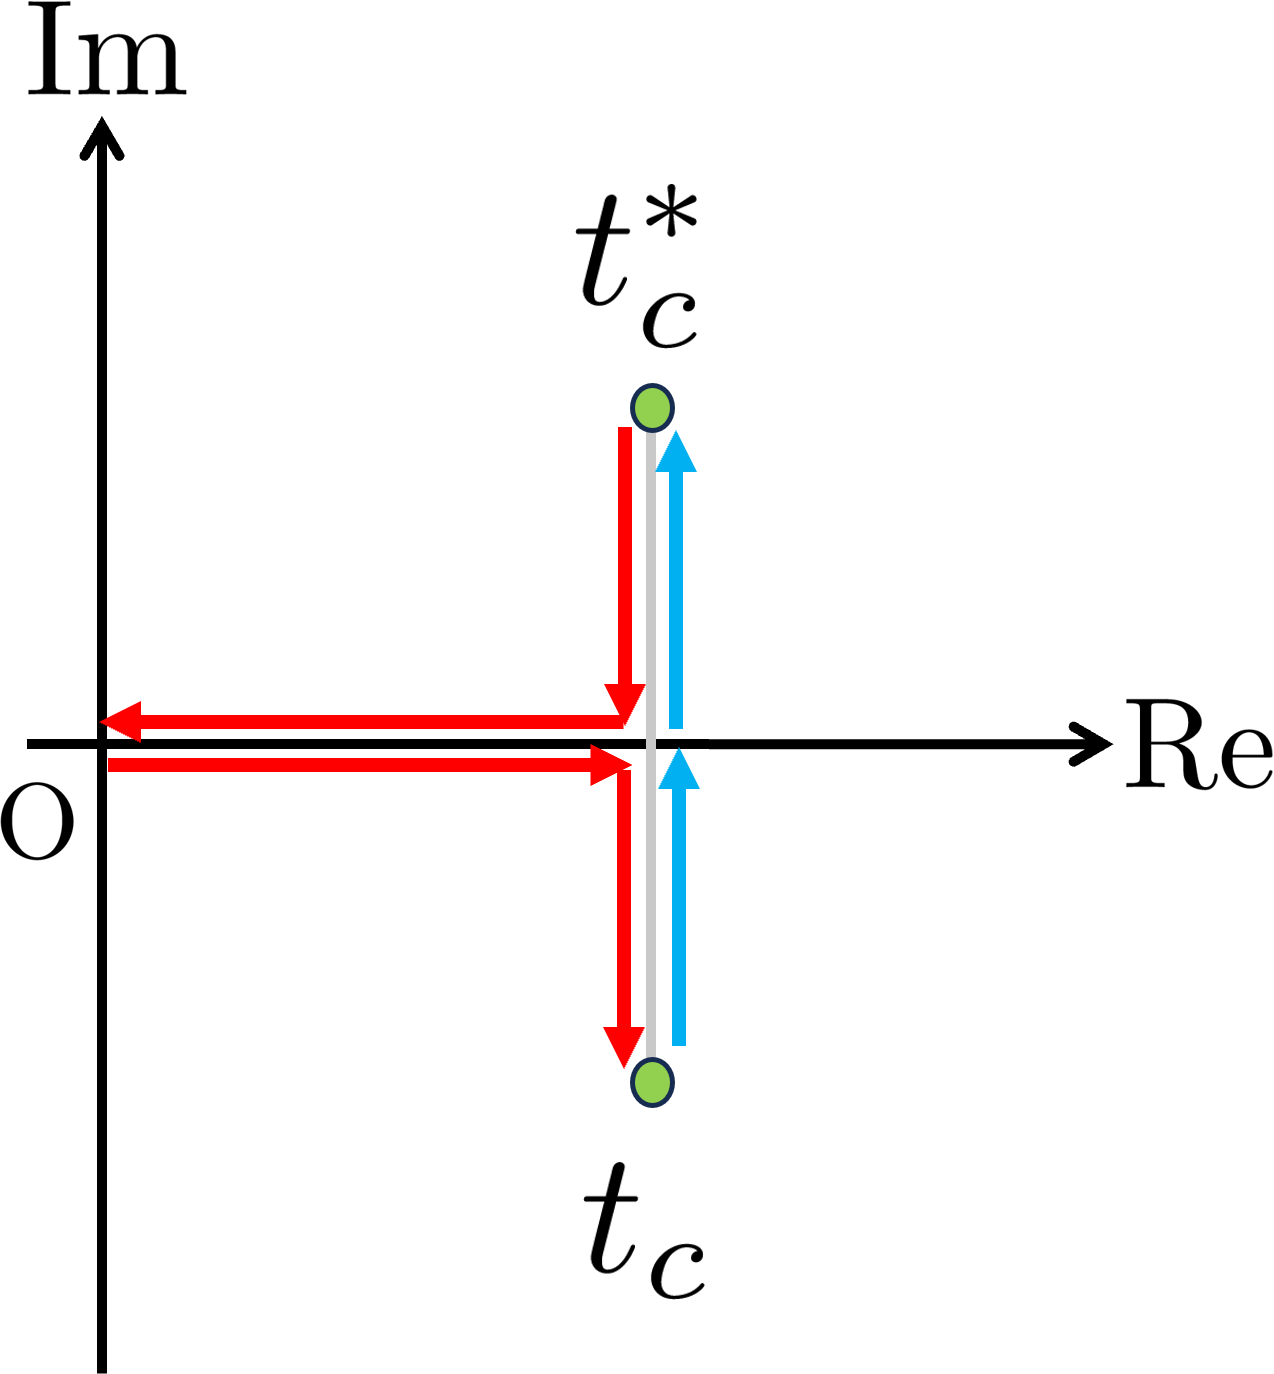
\includegraphics[scale=0.5]{figures/solidangle_GP.png}
  \caption{複素積分(\ref{gamma_g_solid})の経路.赤い線は第1 Riemann面,青い線は第2 Riemann面における経路を表す.また,$t_c$と$t_c^*$を結ぶ緑の線は切断(cut)である.}
  \label{fig:solidangle_GP}
\end{figure}



最後に,$\Gamma_g$の性質を4種類挙げる\cite{Berry1990}.
  \begin{enumerate}
    \item $H(t) = 0$となる$t$が存在するとき,$\Gamma_g = 0$
    \item 時間反転\footnote{$t \rightarrow -t$という変換のこと.}により$\Gamma_g$の符号が変わる
    \item 逆向きの遷移\footnote{今の場合は$|\phi_2(t) \rangle$から$|\phi_1(t) \rangle$への遷移のこと.}で$\Gamma_g$の符号が変わらない
    \item パラメータ空間の軸回りの$\pi$回転にHamiltonianが不変ならば$\Gamma_g = 0$
  \end{enumerate}
特に,性質4は後の議論で重要になる.

\section{Landau-Zener遷移}
Landu-Zener(LZ)遷移\footnote{Majorana,St\"{u}ckelbergの貢献を強調するために,LZMS遷移と呼ぶこともある\cite{Ivakhnenko}.}は,非断熱遷移のもっとも簡単な例である.Landau-Zener遷移が行われる系をLandau-Zener(LZ)モデルと呼ぶ\cite{Zener}.これは,原子の非弾性衝突の確率や磁場における粒子のスピン遷移などの遷移確率を与える重要なモデルである.
LZモデルのHamiltonianは,
\begin{equation}
  \Hat{H}_{\mathrm{LZ}} =
  \begin{pmatrix}
    \varepsilon_0 t & \Delta_0\\
    \Delta_0 & -\varepsilon_0 t
    \label{H_LZ}
  \end{pmatrix}
  \quad (\varepsilon_0 > 0)
\end{equation}
で定義される.ここで,$\varepsilon_0 t$はエネルギーバイアス(energy bias),$\Delta_0$は最小エネルギーギャップ(minimal energy gap)と呼ぶ.また,$\Delta_0 = 0$のときの,Hamiltonian(\ref{H_LZ})についての固有値方程式における固有値を,透熱エネルギー(diabatic energy)と呼ぶ.さらに,それぞれの固有値に属する規格直交化された固有関数を透熱状態(diabatic state)と呼び,属する固有値が小さい順に,$|1\rangle,|2\rangle$で表す\footnote{透熱状態の組を透熱基底と呼ぶ.透熱基底は,断熱基底と同様に完全系をなす.}.


このモデルにおける断熱エネルギーの時間変化を示したのが図\ref{fig:LZ}である.2つの透熱エネルギーが等しくなる部分を準位交差(level crossing)と呼ぶ.また,2つの断熱エネルギーの差がもっとも小さくなる部分では,断熱エネルギーが互いに反発しているように見える.この現象を準位反発(avoided crossing)と呼ぶ.断熱遷移の場合は.初期状態が$| \phi_2(t)\rangle$である系は,準位交差の後も$|\phi_2(t)\rangle$に留まる\footnote{詳しくは第\ref{AT}章を見よ.}.一方,LZ遷移では,準位交差時に状態$|\phi_1(t) \rangle$へ遷移する可能性がある.

\begin{figure}[htbp]
  \centering
  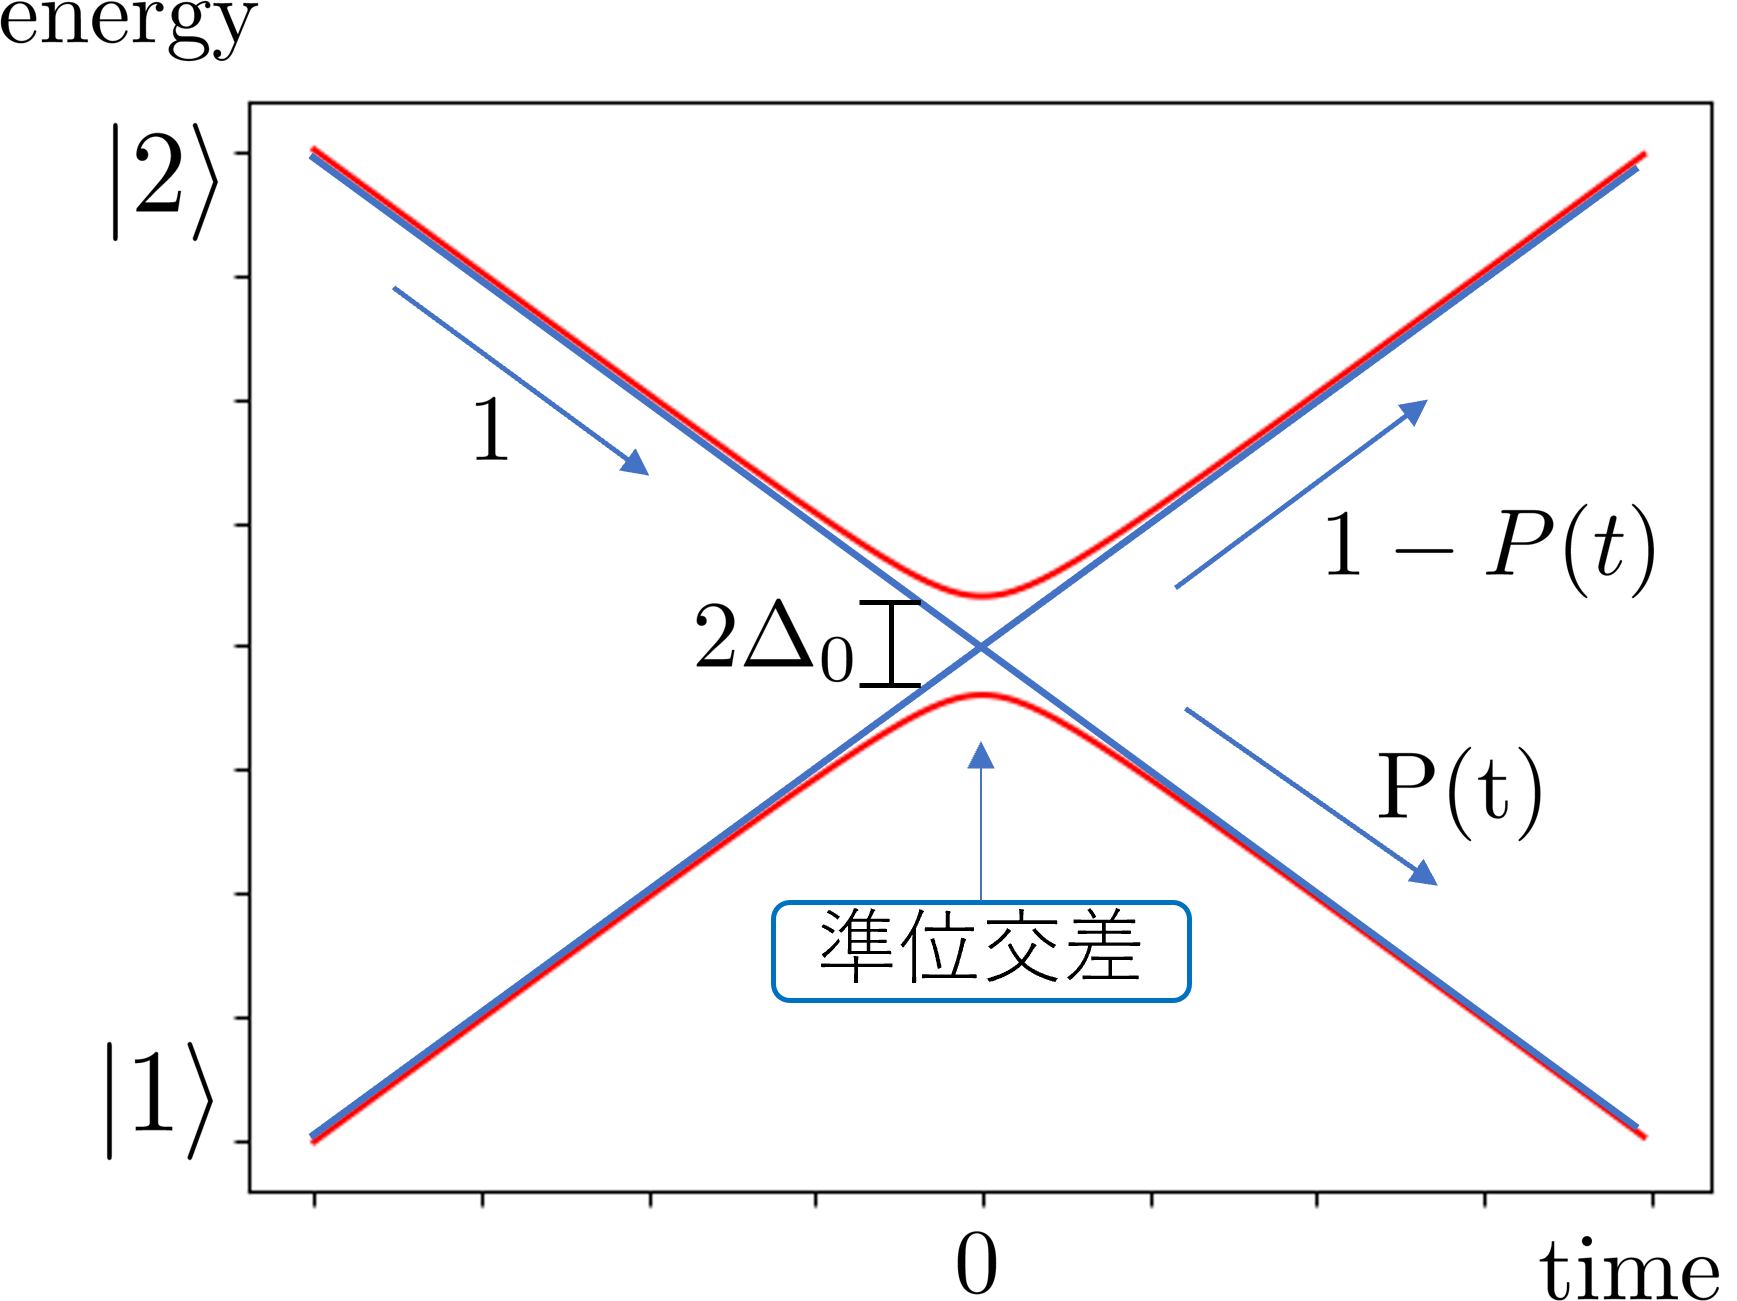
\includegraphics[scale=0.5]{figures/LZ.png}   
  \caption{Landau-Zenerモデルにおける断熱エネルギーの時間変化.赤い線は断熱エネルギー,青い線は透熱エネルギーを示している.$t=0$における断熱エネルギー差は$2\Delta_0$である.}
  \label{fig:LZ}
\end{figure}


この系における$|\phi_2(t)\rangle$から$|\phi_1(t)\rangle$へ遷移する確率$P_{\mathrm{LZ}}$は,
\begin{equation}
  P_{\mathrm{LZ}} = \exp \left(-\frac{\pi \Delta_0^2}{\hbar \varepsilon_0 } \right) 
\end{equation}
であることが知られている.これをLandau-Zener公式と呼ぶ.


また,Pauli行列を基底とするパラメータ空間に,LZモデルのHamiltonian $\Hat{H}_{\mathrm{LZ}}$を描写すると,図\ref{fig:LZ_Pauli}となる.図\ref{fig:LZ_Pauli}および$\Gamma_g$の性質4より,LZモデルでは,幾何学的位相の効果は得られない.

\begin{figure}
  \centering
  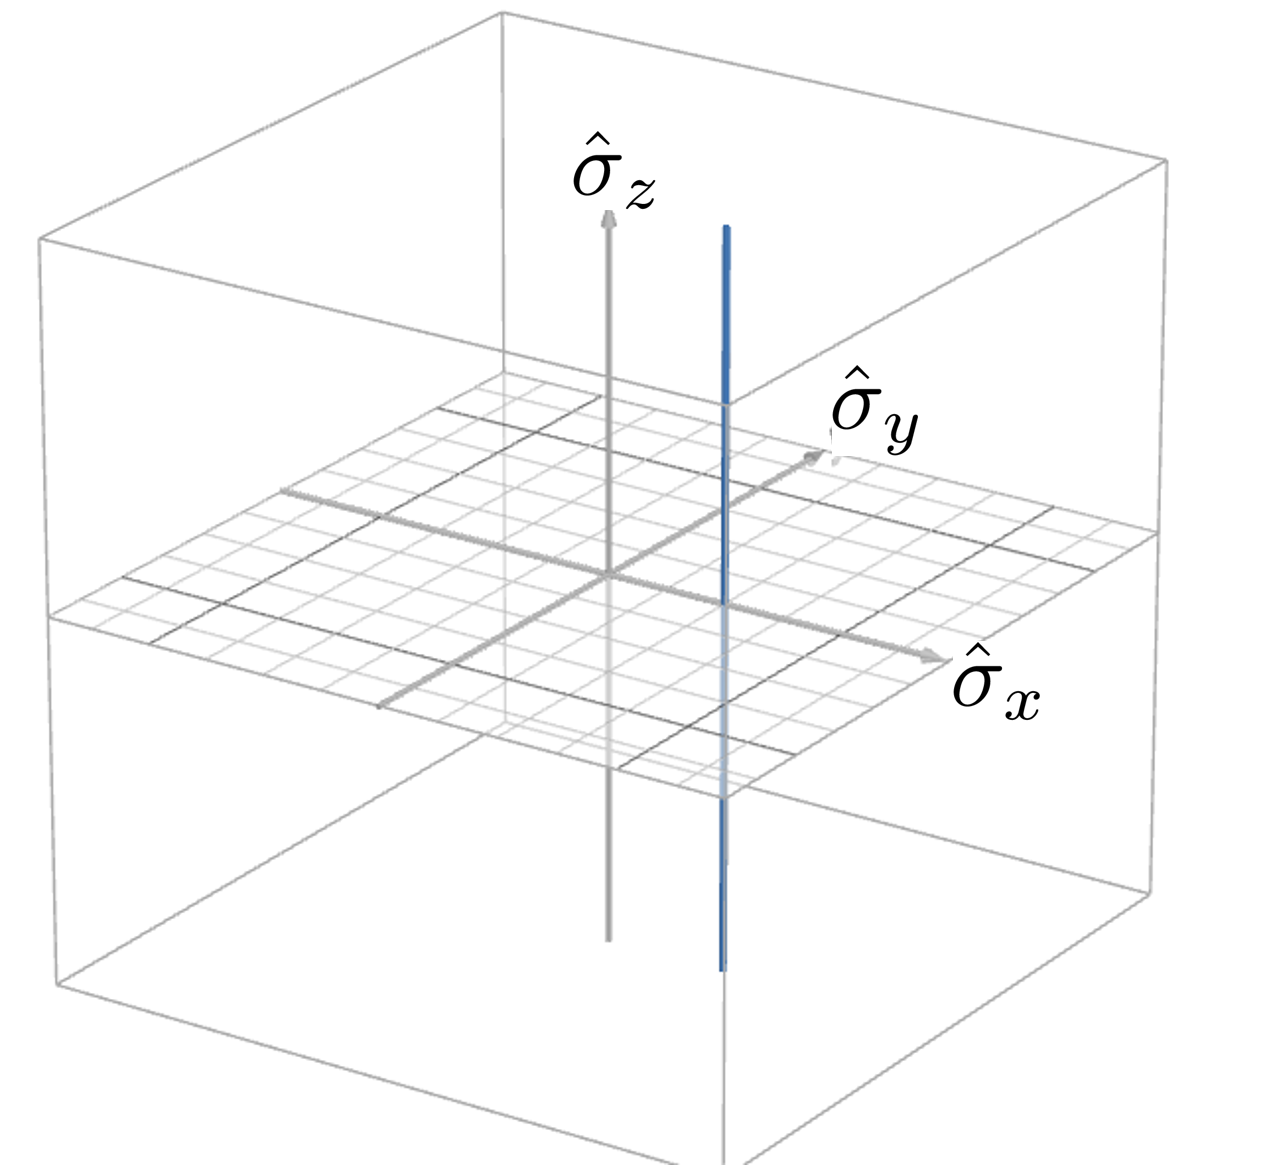
\includegraphics[scale=0.7]{figures/LZ_Pauli.png}
  \caption{Pauli行列を基底とするパラメータ空間におけるLZモデルのHamiltonian $\Hat{H}_{\mathrm{LZ}}$の経路}
  \label{fig:LZ_Pauli}
\end{figure}

\section{Twisted Landau-Zener(TLZ)遷移}
幾何学的位相の効果を具体的に調べるために,BerryはTwisted Landau-Zener(TLZ)モデルを考案した\cite{Berry1990}.TLZモデルのHamiltonianは,
\begin{equation}
 \Hat{H}_{\mathrm{TLZ}} =\Delta_0 \cos \phi(t) \Hat{\sigma}_x + \Delta_y \sin \phi(t) \Hat{\sigma}_y + \varepsilon_0 t \Hat{\sigma}_z
\end{equation}
である\footnote{Berryが提唱したTLZモデルは,厳密には$\Delta_0 = \Delta_y$の場合に限定される.ここでは,$x$成分と$y$成分のパラメータをそれぞれ自由に決められるようにしている.}.ただし,$\Delta_y$は任意の定数,$\phi(t)$は任意の$t$の関数,$t = \delta \tau$である.


LZモデルと同様に,Pauli行列を基底としたパラメータ空間に$H_{\mathrm{TLZ}}$を描写すると,図\ref{fig:uniform_helix}および図\ref{fig:winding_helix}のようになる.これらの図および$\Gamma_g$の性質4より,$\phi(t) \propto t$のように$\phi(t)$が奇関数のときは幾何学的位相の効果は得られない.一方,$\phi(t) \propto t^2$のように$\phi(t)$が偶関数のときは幾何学的位相の効果を得られる.

\begin{figure}[htbp]
  \centering
  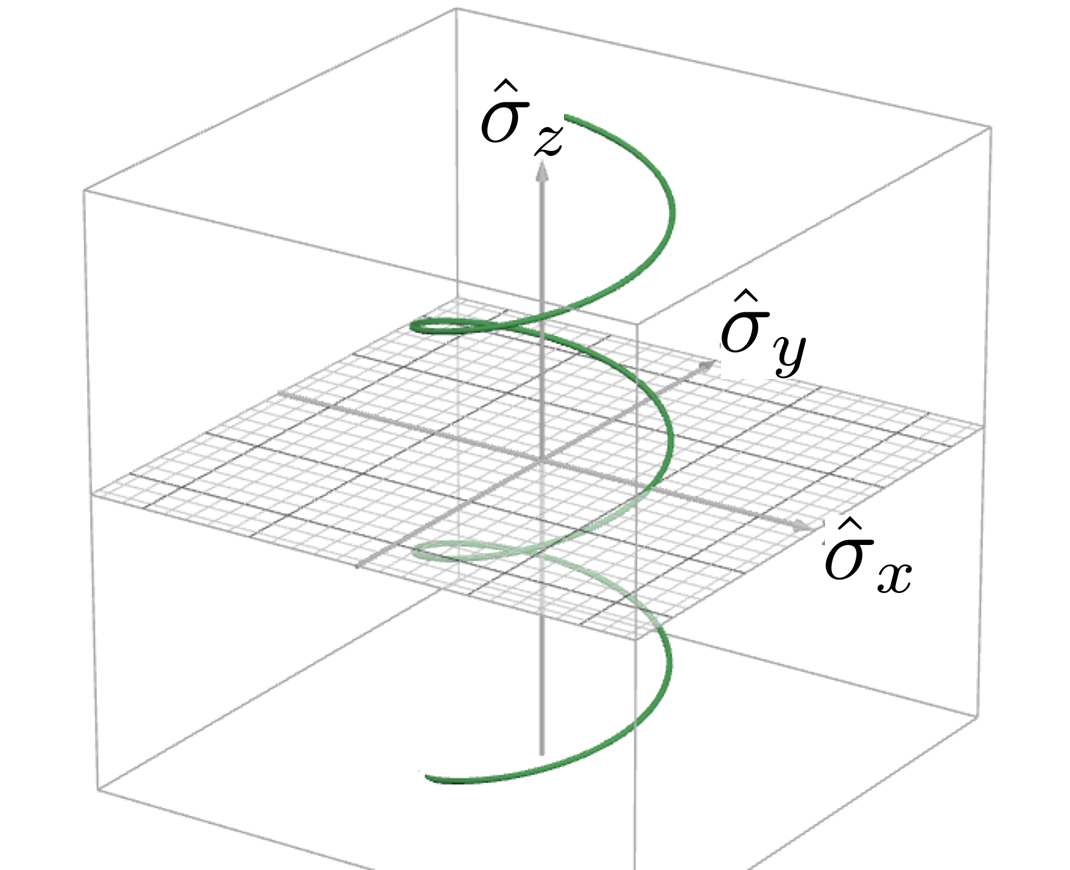
\includegraphics[scale=0.8]{figures/uniform_helix.png}
  \caption{$\phi(t) \propto t$における$H_{\mathrm{TLZ}}$の経路.この図形をuniform helixと呼ぶ.}
  \label{fig:uniform_helix}
\end{figure}

\begin{figure}[htbp]
  \centering
  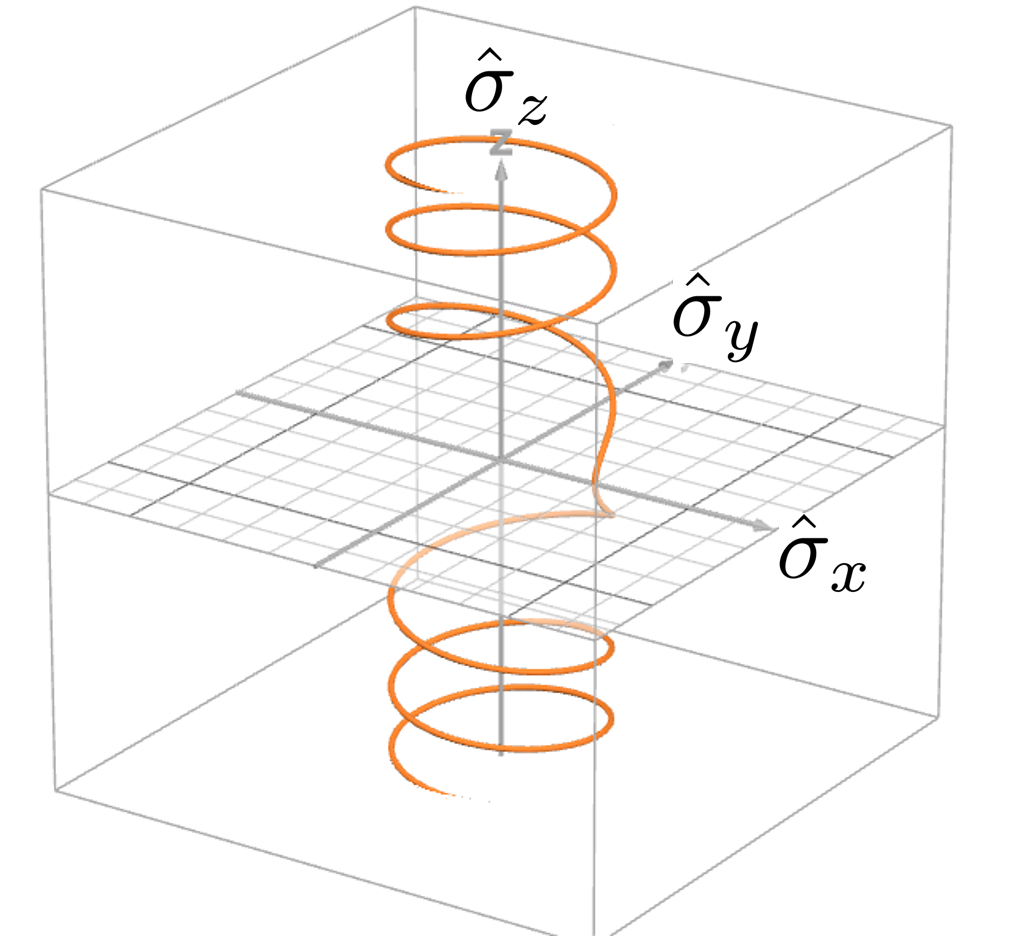
\includegraphics[scale=0.8]{figures/winding_helix.png}
  \caption{$\phi(t) \propto t^2$における$H_{\mathrm{TLZ}}$の経路.この図形をwinding-unwinding helixと呼ぶ.}
  \label{fig:winding_helix}
\end{figure}

$\phi(t) \propto t^2$の場合について,詳しく見てみよう.$\Delta_y = \frac{1}{2} \kappa_g \varepsilon_0^2$として$t^2$の項まで展開すると,
\begin{equation}
  \Hat{H}_{\mathrm{TLZ}} = \Delta_0 \, \Hat{\sigma}_x + \frac{1}{2} \kappa_g \varepsilon_0^2 (\delta \tau)^2 \, \Hat{\sigma}_y + \varepsilon_0 \delta \tau \, \Hat{\sigma}_z
\end{equation}
となる.ただし,$\kappa_g$は${\tau}=0$における測地曲率である.


ここで,測地曲率について説明しよう.ある曲面$S$を通る曲線$C(s)$があるとする.この曲線$C(s)$の1階微分および2階微分
\begin{equation}
  \frac{d C(s)}{d s}, \frac{d^2 C(s)}{d s^2}
\end{equation}
をそれぞれ曲線の接ベクトル,曲率ベクトルと呼ぶ.また,曲面$S$の法ベクトルを$\bm{n}(s)$とする.このとき,
\begin{equation}
  \kappa_g =  \left(\bm{n}(s) \times \frac{d C(s)}{d s} \right)\cdot \frac{d^2 C(s)}{d s^2}
\end{equation}
を測地曲率と呼ぶ.TLZモデルにおける測地曲率のイメージ図を図\ref{fig:geodesic_curvature}で示しておく.青い矢印で表される曲率ベクトルを灰色の接平面に射影したときの長さが測地曲率である.


\begin{figure}[hpbt]
  \centering
  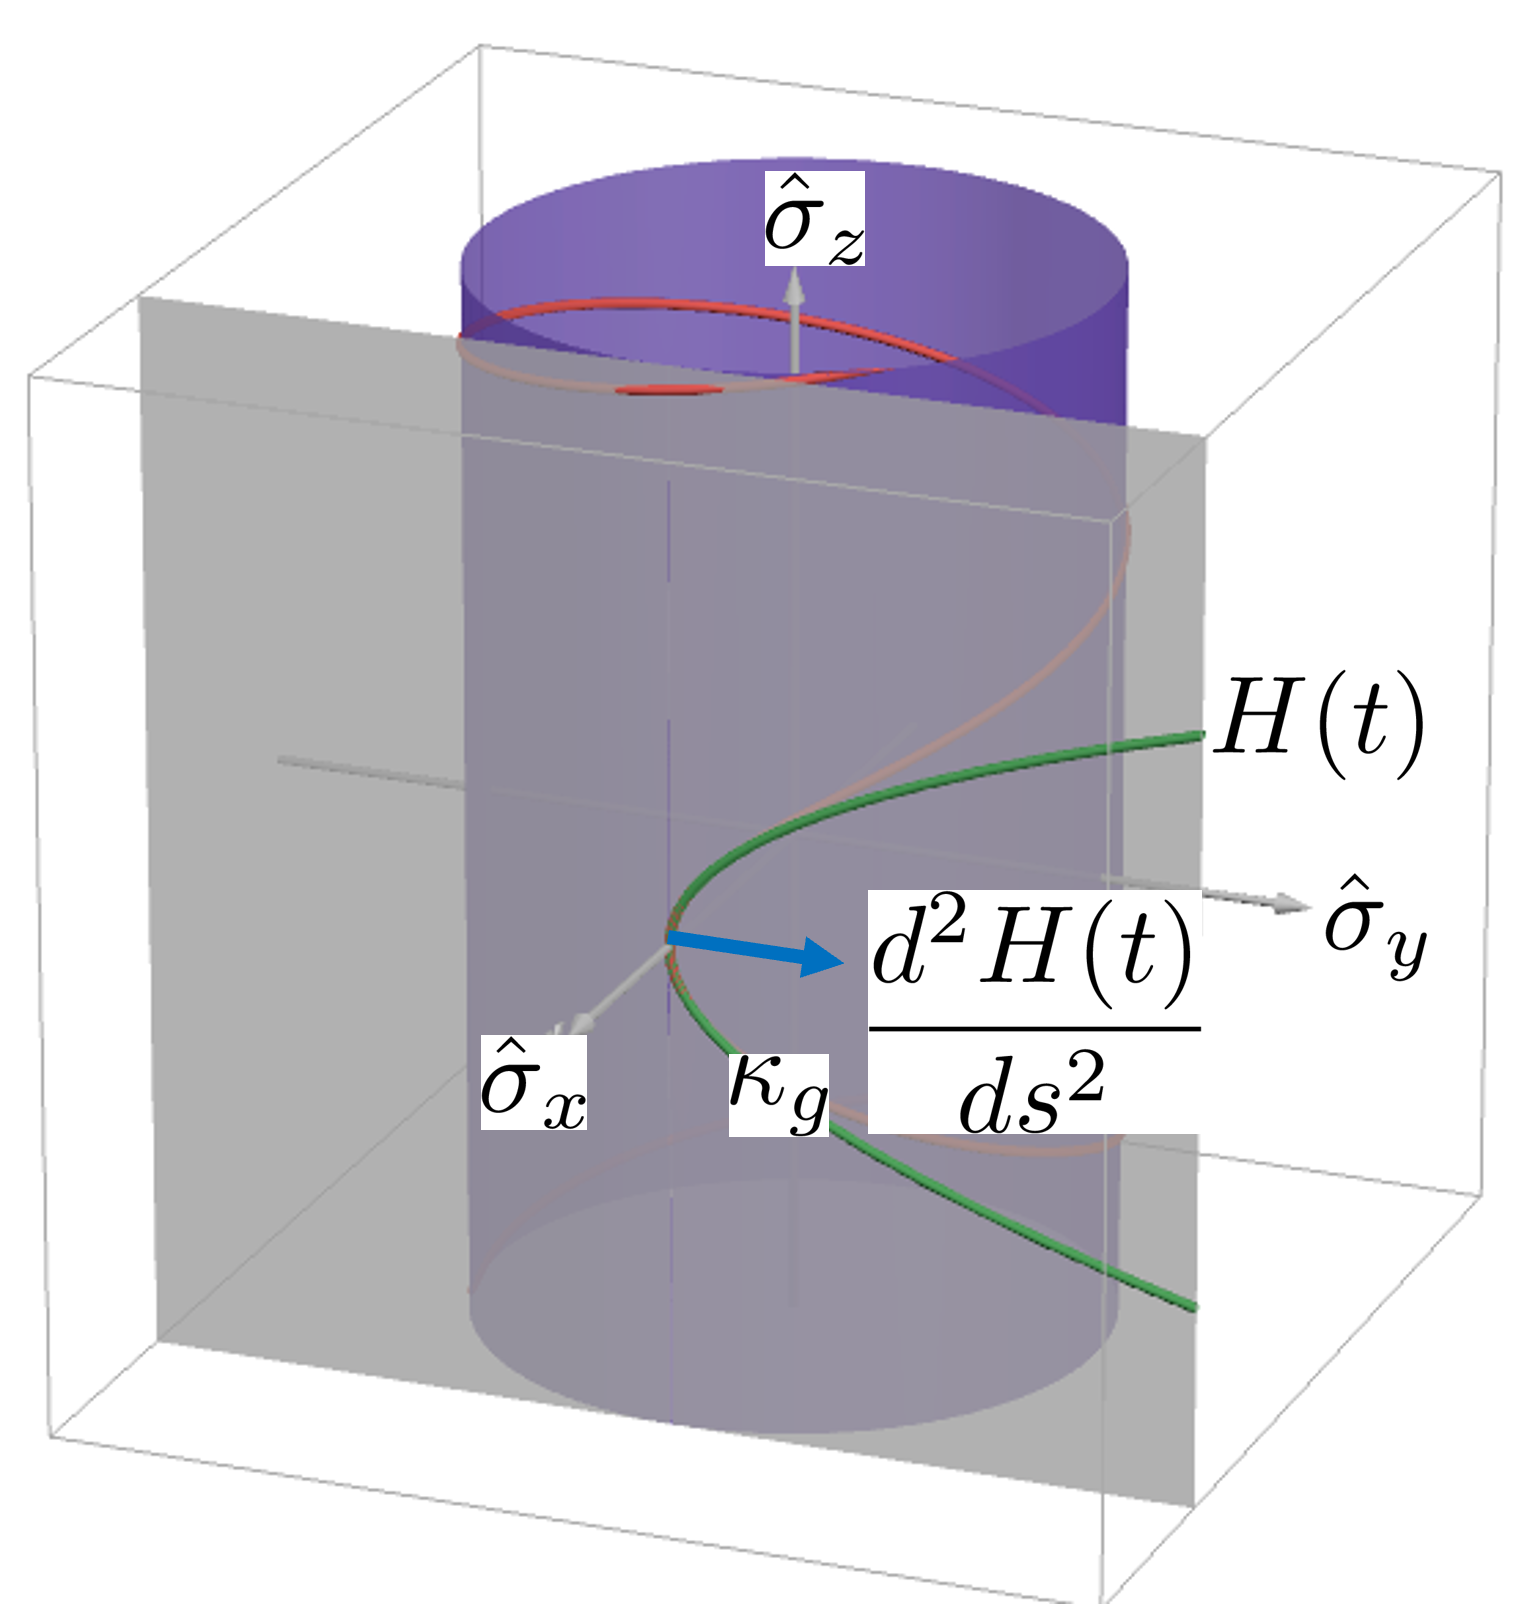
\includegraphics[scale=0.7]{figures/geodesic_curvature.png}
  \caption{TLZモデルにおける測地曲率のイメージ図.オレンジ線がTLZモデルの経路である.緑線はTLZモデルを2次展開したときの経路である.青矢印は,TLZモデルにおける曲率ベクトルである.紫色の面はTLZモデルの経路が通る曲面である.灰色の面は${\tau}=0$における紫色の面の接平面である.}
  \label{fig:geodesic_curvature}
\end{figure}


このモデルにおける遷移確率は,
\begin{equation}
  P(\delta) = \exp \left[-\pi \frac{(\Delta_0 -\frac{\kappa_g \varepsilon_0 \delta}{4})^2}{\varepsilon_0 |\delta|}\right] \label{TLZ_TP}
\end{equation}
となることが知られている\cite{Oka}.次節でこの遷移確率を導出する.また,QGPを用いて書き換えると,
\begin{equation}
  P(\delta) = \exp \left[-\frac{\pi}{4\varepsilon_0 |\delta|} \left(\Delta_0 + \frac{\delta \Delta_{21}}{2}\right)\right]
\end{equation}
となる.この式は,Landau-Zenerモデルにおいて,
\begin{equation}
  \Delta_0 \rightarrow \Delta_0 + \frac{\delta \Delta_{21}}{2}
\end{equation}
と置き換えた形になっている.そのため,幾何学的効果は,エネルギーギャップをシフトさせることを明示的に教えてくれる.$P(\delta)$のグラフは図\ref{fig:Curvature_Effect}のようになる.LZモデルの場合は,$P(\delta)$のグラフは$\delta$の符号に対称である.一方,TLZモデルの場合は,$P(\delta)$のグラフが$\delta$の符号に非対称になる.この非対称性を,整流作用(rectification)と呼ぶ.特に,$P(\delta)=1$となる$\delta$が存在することが重要である.この現象を完全トンネル(perfect tunneling)という.

\begin{figure}
  \centering
  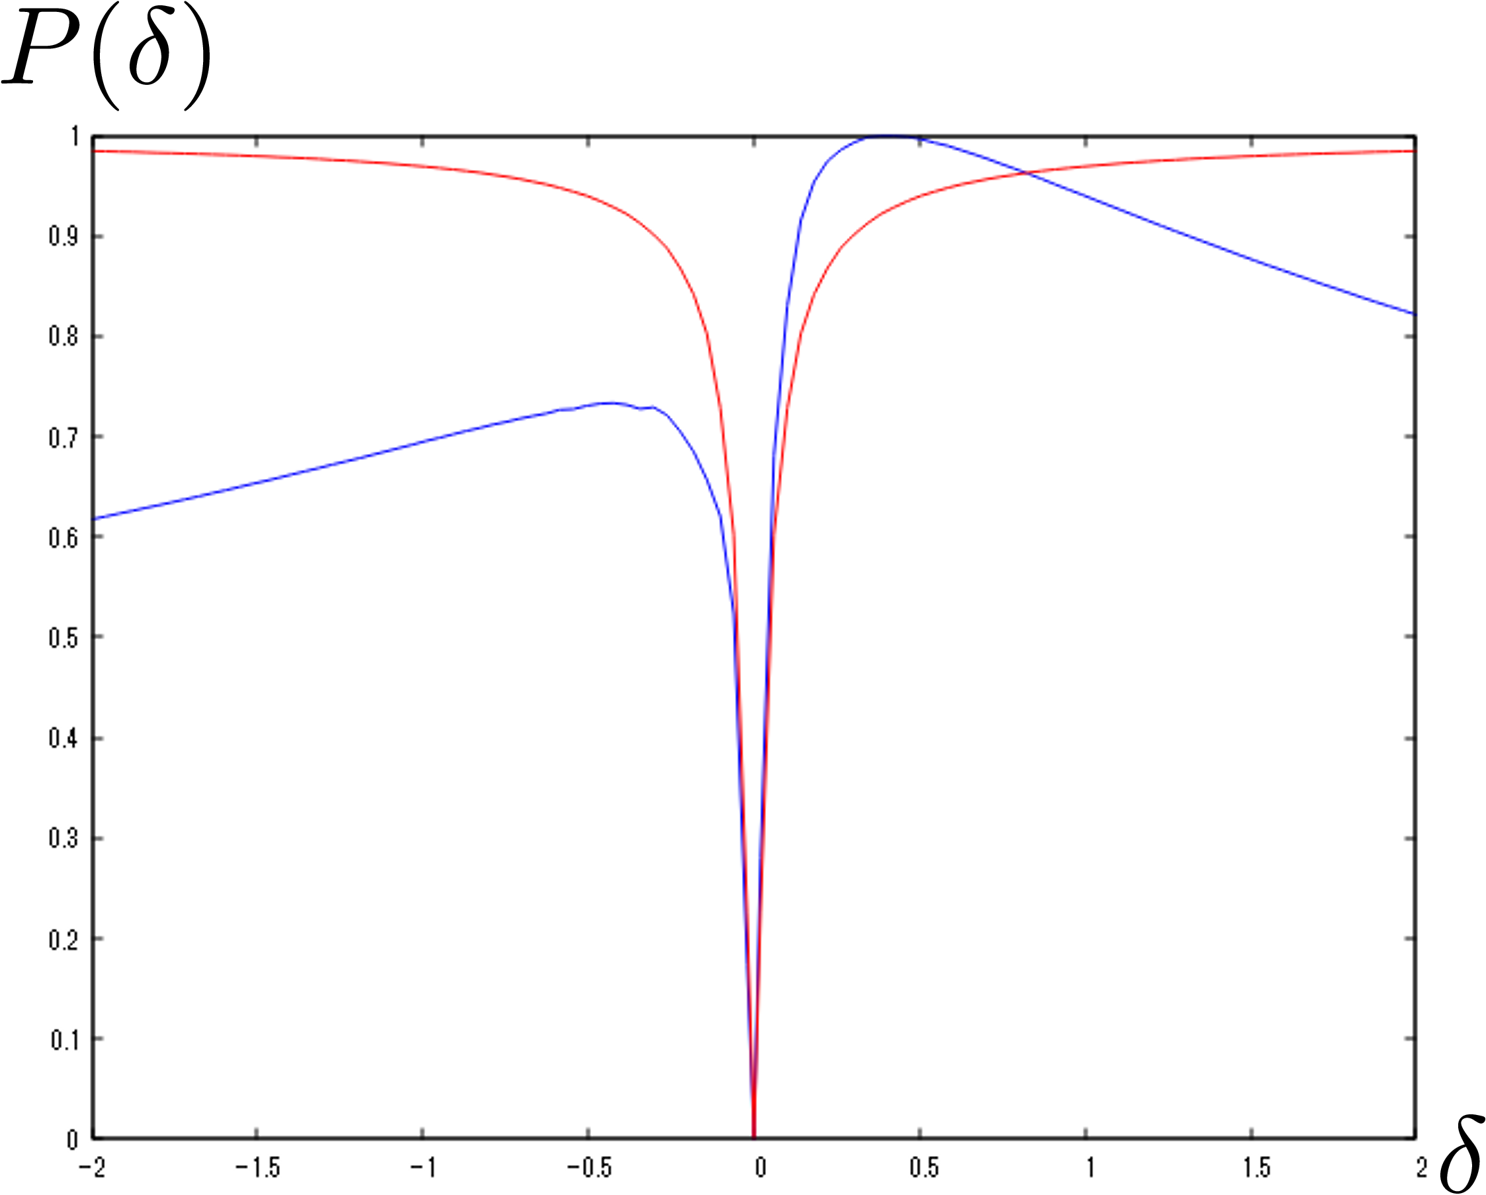
\includegraphics[scale=0.7]{figures/Curvature_Effect.png}
  \caption{$P(\delta)$の$\delta$依存性を示したグラフ.$\varepsilon_0 = 1, \Delta_0 =0.1$である.また,青い線は$\kappa_g = 1$,赤い線は$\kappa_g = 0$の場合を表す.}
  \label{fig:Curvature_Effect}
\end{figure}

\section{TLZモデルにおける遷移確率の導出}
本節では,式(\ref{TLZ_TP})を導出する.そのために,
\begin{equation}
  \bm{d}(t) := (x(t),y(t),z(t))^T \label{d}
\end{equation}
として,$t=0$における3つの量
\begin{align}
  \bm{r} &:= \frac{\bm{d}(0)}{|\bm{d}(0)|} \label{r}\\
  \bm{t} &:= \frac{\partial_{\tau} \bm{d}(0)}{|\partial_{\tau} \bm{d}(0)|} \label{t}\\
  \bm{n} &:= \bm{r}\times \bm{t} \label{n}
\end{align}
を定義する.$\bm{r}$,$\bm{t}$,$\bm{n}$はそれぞれ動径ベクトル,接ベクトル,法ベクトルである.今の系では,式(\ref{d})が,
\begin{equation}
  \bm{d} =
  \begin{pmatrix}
    \Delta_0\\
    \frac{1}{2} \kappa_g \varepsilon_0^2 t^2\\
    \varepsilon_0 t\\
  \end{pmatrix}
\end{equation}
である場合を考えればよい.このとき,動径ベクトル(\ref{r}),接ベクトル(\ref{t}),法ベクトル(\ref{n})はそれぞれ,
\begin{equation}
  \bm{r} =
  \begin{pmatrix}
    1\\
    0\\
    0\\
  \end{pmatrix}, \quad
  \bm{t} =
  \begin{pmatrix}
    0\\
    0\\
    1\\
  \end{pmatrix}, \quad
  \bm{n} =
  \begin{pmatrix}
    0\\
    1\\
    0\\
  \end{pmatrix}
\end{equation}
となる.ここで,
\begin{align}
  a(t) &:= \bm{d}(t)\cdot \bm{t} = z\\
  b(t) &:= \sqrt{|\bm{d}(t)|^2-a(t)^2} = \sqrt{x^2+y^2}
\end{align}
を定義すると,
\begin{equation}
  \Hat{U}^{\dagger} \Hat{H} \Hat{U}
  = \left( a(t)\bm{t} + b(t) \bm{r} \right) \cdot \Hat{\bm{\sigma}}
\end{equation}
と表せる.したがって,
\begin{align}
  a(t)
  &= 
  \begin{pmatrix}
    \Delta_0\\
    \frac{1}{2} \kappa_g \varepsilon_0^2 t^2\\
    \varepsilon_0 t\\
  \end{pmatrix}
  \cdot
  \begin{pmatrix}
    1\\
    0\\
    0\\
  \end{pmatrix}\\
  &=
  \Delta_0,\\
  b(t)
  &=
  \sqrt{\left|
  \begin{pmatrix}
    \Delta_0\\
    \frac{1}{2} \kappa_g \varepsilon_0^2 t^2\\
    \varepsilon_0 t\\
  \end{pmatrix}
  \right|^2 -\Delta_0^2}\\
  &= \sqrt{(\varepsilon_0 t)^2 + (\frac{1}{2} \kappa_g \varepsilon_0^2 t^2)^2}\\
  &\approx \varepsilon_0 t (1+ (\frac{1}{2} \kappa_g \varepsilon_0 \tau)^2)^{\frac{1}{2}}\\
  &= \varepsilon_0 t + O(t^3),\\
  \phi(t)
  &= \arctan \frac{\kappa_g \varepsilon_0 t}{2} \label{phi_arc}
\end{align}
である.また,式(\ref{phi_arc})の両辺を$t$で微分すると,
\begin{align}
  \partial_t \phi(t)
  &= \frac{\frac{\kappa_g \varepsilon_0 t}{2}}{1+(\frac{\kappa_g \varepsilon_0 t}{2})^2}\\
  &= \frac{\kappa_g \varepsilon_0}{2} (1-(\frac{\kappa_g \varepsilon_0 t}{2})^2)^{-1}\\
  &= \frac{\kappa_g \varepsilon_0}{2} + O(t^2)
\end{align}
となる.さらに,断熱エネルギー(\ref{E_LZ})は,
\begin{equation}
  E_{\mathrm{LZ}_2}(t) \approx  \sqrt{\left(\Delta_0 - \left(\frac{\kappa_g \varepsilon_0 \delta }{4}\right) \right)^2 + (\varepsilon_0 t)^2}
\end{equation}
である.$E_{\mathrm{LZ}_2}(t_c) = 0$となる,断熱エネルギー$E_{\mathrm{LZ}_2}(t_c)$の零点$t_c$は,
\begin{equation}
  t_c = \frac{i}{\varepsilon_0} \left( \Delta_0 - \left(\frac{\kappa_g \varepsilon_0 \delta}{4}\right) \right)
\end{equation}
と定まる.よって,TLZ遷移における遷移確率(\ref{P_nt})は,
\begin{align}
  P
  &\approx \exp \left(\frac{4}{|\delta|} \mathrm{Im} \int_0^{t_c} \sqrt{\left( \left( \Delta_0 - \left(\frac{\kappa_g \varepsilon_0 \delta }{4}\right) \right)^2 + (\varepsilon_0 t)^2 \right)} dt \right)\\
  &= \exp \left(\frac{4}{|\delta|} \int_0^{\frac{1}{\varepsilon_0} (\Delta_0 - \frac{\kappa_g \varepsilon_0 \delta}{4})} \sqrt{\left( \left( \Delta_0 - \left(\frac{\kappa_g \varepsilon_0 \delta}{4} \right)\right)^2 - (\varepsilon_0 t)^2 \right)} dt \right)
\end{align}
である.ここで,積分を実行するために,変数変換
\begin{equation}
  t = \frac{1}{\varepsilon_0} \left(\Delta_0 - \frac{\kappa_g \varepsilon_0 \delta}{4} \right) \cos \varphi
\end{equation}
を行うと,
\begin{align}
  P
  &= \exp \left(\frac{4}{|\delta|} \int_{\frac{\pi}{2}}^0 \sqrt{\left(\Delta_0 - \left(\frac{\kappa_g \varepsilon_0 \delta}{4}\right) \right)^2 (1-\cos^2\varphi)} \frac{1}{\varepsilon_0} \left( \Delta_0 - \frac{\kappa_g \varepsilon_0 \delta}{4} \right) (-\sin \varphi) d\varphi \right)\\
  &= \exp \left(-\frac{4}{\varepsilon_0 |\delta|} \left(\Delta_0 - \frac{\kappa_g \varepsilon_0 \delta}{4} \right) ^2\int_0^{\frac{\pi}{2}} \sin^2\theta d\theta \right)\\
  &= \exp \left(-\frac{4}{\varepsilon_0 |\delta|} \left(\Delta_0 - \frac{\kappa_g \varepsilon_0 \delta}{4} \right) ^2 \frac{\pi}{4} \right)\\
  &= \exp \left(-\frac{\pi}{4} \frac{(2\Delta_0-\frac{\kappa_g \varepsilon_0 \delta}{4})^2}{\varepsilon_0 |\delta|} \right)\\
  &= \exp \left[-\pi \frac{(\Delta_0 -\frac{\kappa_g \varepsilon_0 \delta}{4})^2}{\varepsilon_0 |\delta|}\right]
\end{align}
となり,式(\ref{TLZ_TP})が示された.